% Included by reports/main.tex (no preamble in module files).
\section{Module 4 --- Liquidity Provision Analytics}
\label{sec:module4}

\subsection{Objective and Scope}
\label{subsec:m4-objective}
This module studies the USDC/WETH Uniswap V3 pool from the liquidity provider (maker) perspective. We construct five synthetic representative LP positions sized at \$100{,}000 at the start of the study window, then decompose performance into (i) fee income earned while the position is in-range and (ii) impermanent loss (IL) relative to a HODL benchmark holding the same initial token quantities.

\paragraph{Pool configuration used in this module.}
\begin{itemize}
    \item Protocol: Uniswap V3
    \item Pair: USDC/WETH
    \item Fee tier: 0.05\% (5 bps)
    \item Contract: \texttt{0x88e6A0c2dDD26FEEb64F039a2c41296FcB3f5640}
\end{itemize}

\subsection{Data Inputs}
\label{subsec:m4-data}
\paragraph{Inputs used.}
\begin{itemize}
    \item \texttt{slot0\_snapshots.parquet}: daily snapshot blocks with mid-price (USDC per WETH) and current tick.
    \item \texttt{swap\_events.parquet}: per-swap amounts, tick after swap, and active liquidity used to compute fee shares.
\end{itemize}

\subsection{Task 4.1 --- Representative LP Positions}
\label{subsec:m4-task41}
We define five synthetic positions, all entered at the first snapshot and exited at the last snapshot. Positions P1--P4 are symmetric price bands around the entry price, while P5 is full range (V2-equivalent).

\paragraph{Position set (constructed at entry).}
\begin{table}[t]
    \centering
    \caption{Representative LP positions at entry (notional \$100{,}000).}
    \label{tab:m4-positions}
    \begin{tabular}{lrrrr}
        \hline
        ID & Tick lower & Tick upper & Initial USDC & Initial WETH \\
        \hline
        P1 & 193010 & 193040 & 60{,}254.76 & 9.5874 \\
        P2 & 192970 & 193080 & 52{,}793.93 & 11.3871 \\
        P3 & 192820 & 193230 & 50{,}746.78 & 11.8809 \\
        P4 & 192060 & 194080 & 52{,}320.62 & 11.5013 \\
        P5 & -887270 & 887270 & 50{,}000.00 & 12.0611 \\
        \hline
    \end{tabular}
\end{table}

\paragraph{Liquidity sizing under the \$100{,}000 constraint.}
Let the entry price be $p_0$ (USDC per WETH), with corresponding square-root price $\sqrt{p_0}$. For a range with bounds $(\sqrt{p_a}, \sqrt{p_b})$, Uniswap V3 virtual reserves for liquidity $L$ imply:
\[
x(L) =
\begin{cases}
L\left(\frac{1}{\sqrt{p_a}} - \frac{1}{\sqrt{p_b}}\right), & \sqrt{p_0} \le \sqrt{p_a}, \\
L\left(\frac{1}{\sqrt{p_0}} - \frac{1}{\sqrt{p_b}}\right), & \sqrt{p_a} < \sqrt{p_0} < \sqrt{p_b}, \\
0, & \sqrt{p_0} \ge \sqrt{p_b},
\end{cases}
\qquad
y(L) =
\begin{cases}
0, & \sqrt{p_0} \le \sqrt{p_a}, \\
L(\sqrt{p_0} - \sqrt{p_a}), & \sqrt{p_a} < \sqrt{p_0} < \sqrt{p_b}, \\
L(\sqrt{p_b} - \sqrt{p_a}), & \sqrt{p_0} \ge \sqrt{p_b},
\end{cases}
\]
where $x$ is the amount of token0 (USDC) and $y$ is the amount of token1 (WETH). The entry portfolio value is $V_0(L) = x(L) + p_0\,y(L)$. We solve for $L$ via:
\[
L = \frac{100{,}000}{V_0(1)},
\]
and then compute initial deposits $(x_0, y_0)=(x(L), y(L))$.

\subsection{Task 4.2 --- Fee Income Computation}
\label{subsec:m4-task42}
Fees are computed from first principles by allocating each swap's total fee amount to the synthetic LP in proportion to its liquidity share, but only when the swap occurs while the pool tick is in the position range.

\paragraph{Per-swap fee in USD.}
With fee rate $f=0.0005$, each swap contributes fees in both tokens; in USD terms:
\[
\mathrm{FeeUSD}_i = f\cdot \max(\Delta \mathrm{USDC}_i, 0) + f\cdot \max(\Delta \mathrm{WETH}_i, 0)\cdot p_i,
\]
where $p_i$ is the swap price (USDC per WETH) and the max() operator selects the token deposited into the pool on that swap.

\paragraph{LP share and in-range filter.}
For position $j$ with liquidity $L_j$, for swaps where $\mathrm{tick}_i \in [\mathrm{tick}^{(j)}_{\mathrm{lower}},\mathrm{tick}^{(j)}_{\mathrm{upper}})$, the USD fee attributed is:
\[
\mathrm{FeeUSD}_{i,j} = \mathrm{FeeUSD}_i \cdot \frac{L_j}{\mathrm{ActiveLiquidity}_i}.
\]
We aggregate fees between daily snapshot blocks and report both daily and cumulative fee income time series.

\subsection{Task 4.3 --- Impermanent Loss and Net P\&L}
\label{subsec:m4-task43}
At each daily snapshot $t$ with ETH price $p_t$, we compute:
\[
V_{\mathrm{HODL}}(t) = x_0 + p_t\,y_0,
\qquad
V_{\mathrm{LP}}(t) = x_t + p_t\,y_t,
\qquad
\mathrm{IL}(t) = V_{\mathrm{HODL}}(t) - V_{\mathrm{LP}}(t),
\]
where $(x_t,y_t)$ are the Uniswap V3 virtual reserves implied by the fixed liquidity $L$ and the current price relative to the position range (below, within, or above). Finally, we report a net metric consistent with the project brief:
\[
\mathrm{Net}(t) = \mathrm{CumulativeFees}(t) - \mathrm{IL}(t).
\]

\subsection{Results}
\label{subsec:m4-results}
\begin{figure}[t]
    \centering
    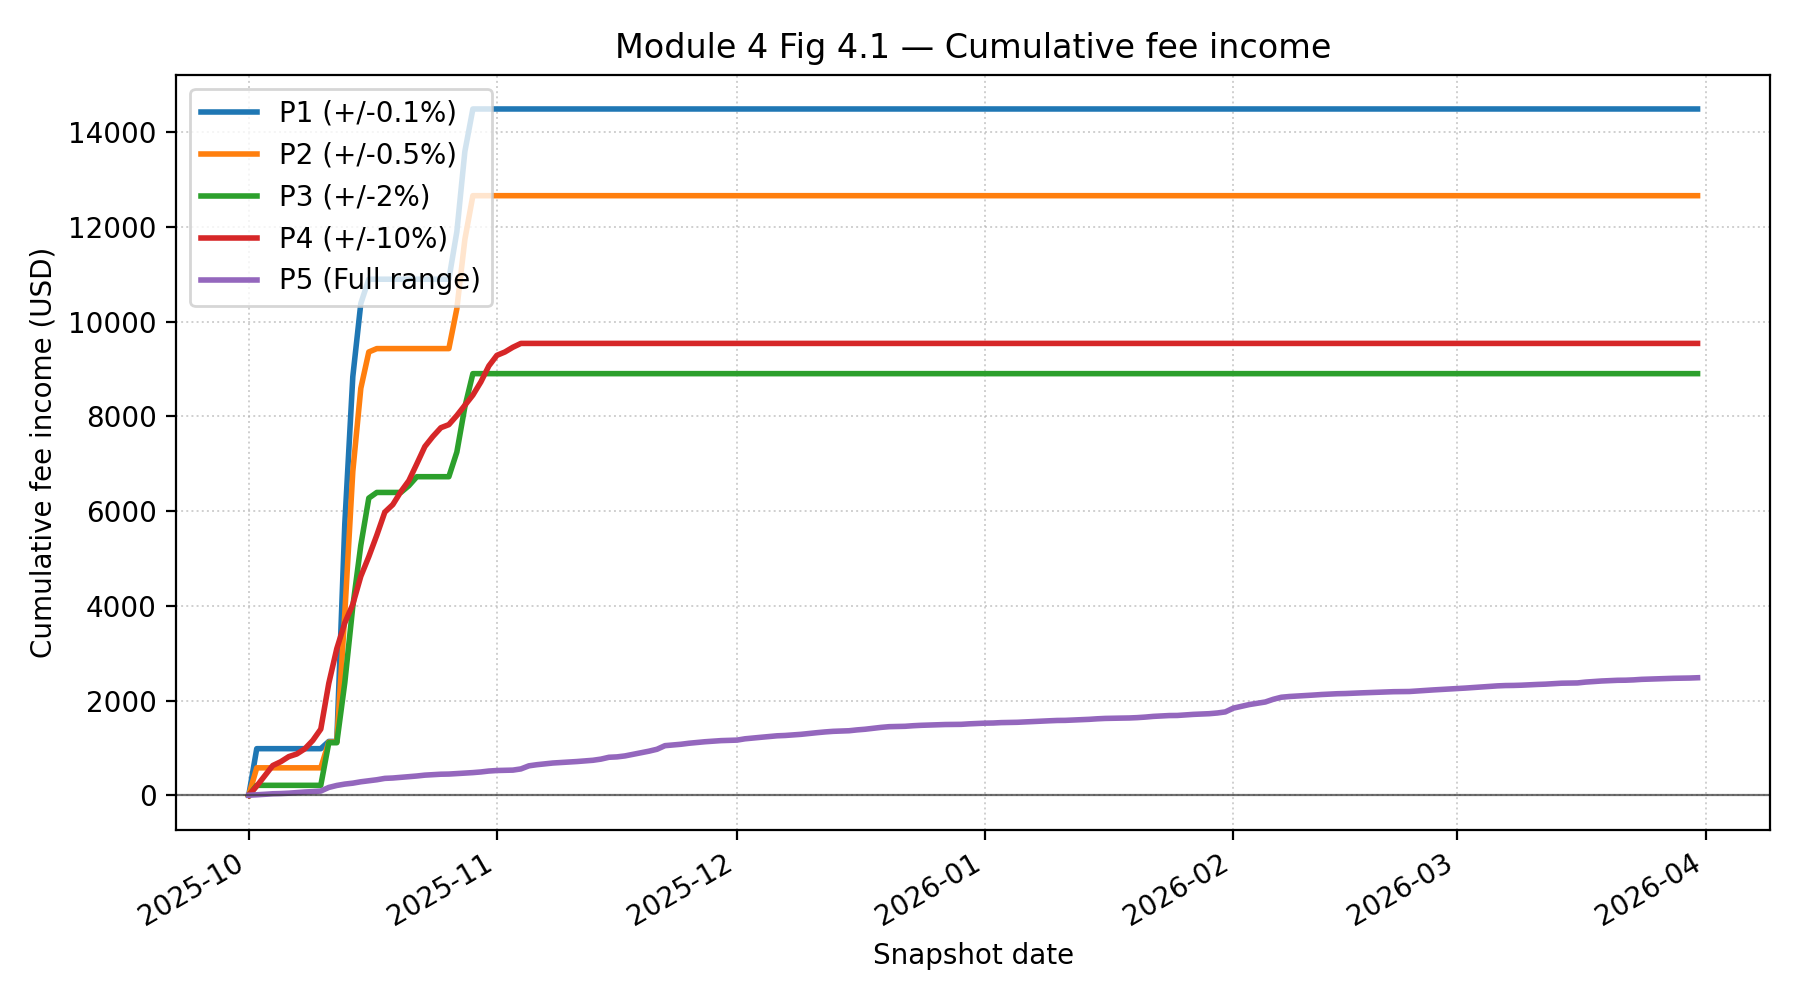
\includegraphics[width=\linewidth]{../data/results/module_4/figures/module4_cumulative_fee_income.png}
    \caption{Fig 4.1 --- Cumulative fee income time series for the five representative LP positions.}
    \label{fig:m4-fees}
\end{figure}

\begin{figure}[t]
    \centering
    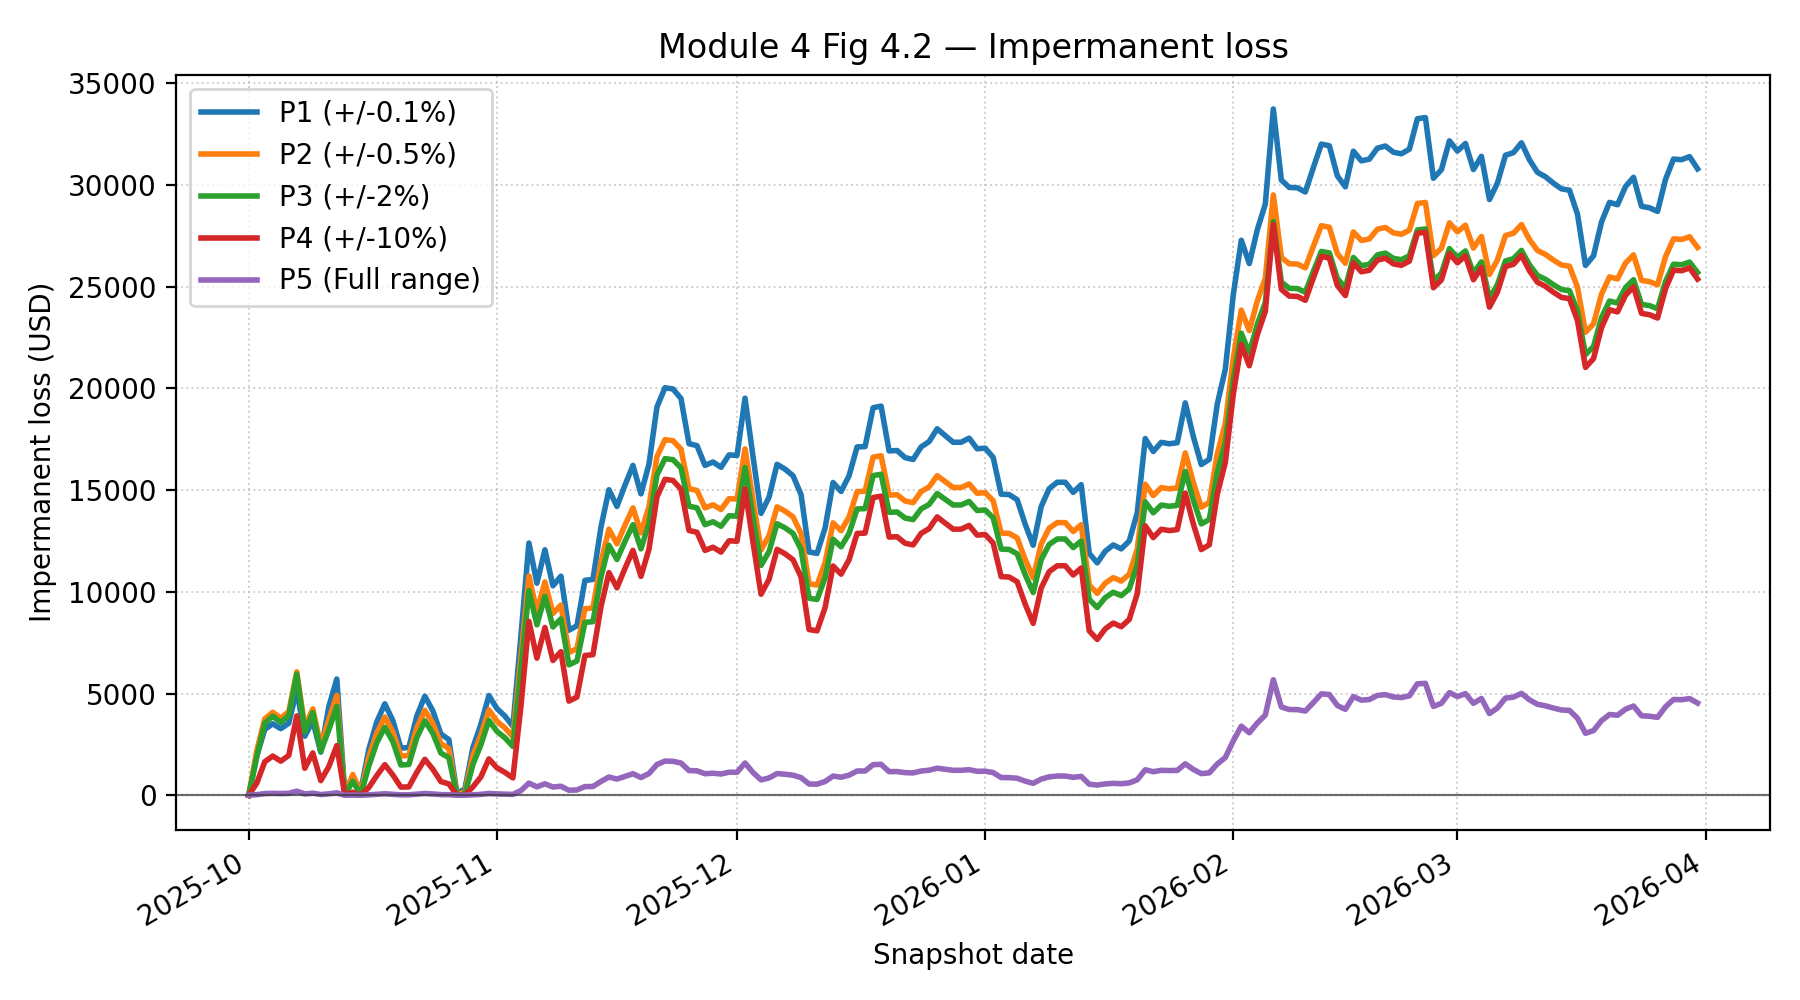
\includegraphics[width=\linewidth]{../data/results/module_4/figures/module4_impermanent_loss.png}
    \caption{Fig 4.2 --- Impermanent loss time series (HODL value minus LP principal value).}
    \label{fig:m4-il}
\end{figure}

\begin{figure}[t]
    \centering
    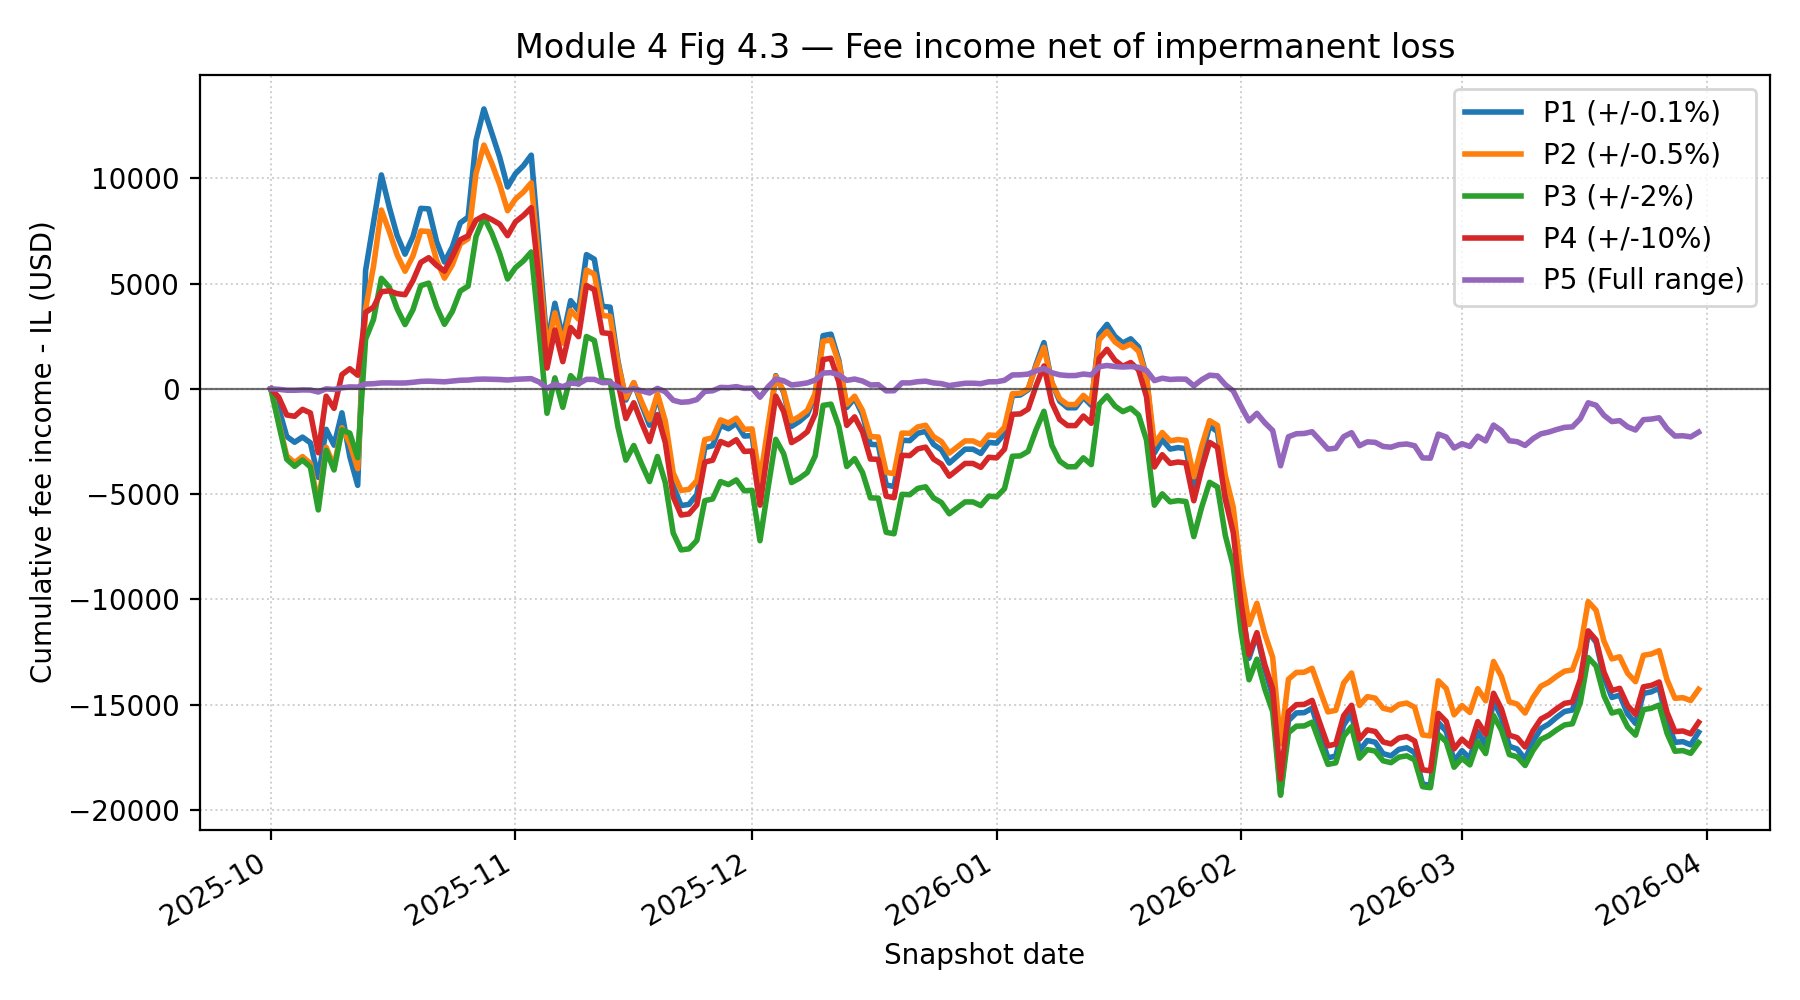
\includegraphics[width=\linewidth]{../data/results/module_4/figures/module4_net_fee_minus_il.png}
    \caption{Fig 4.3 --- Cumulative fee income minus impermanent loss for each position.}
    \label{fig:m4-net}
\end{figure}

\subsection{Module 4 Deliverables Checklist}
\label{subsec:m4-checklist}
\begin{itemize}
    \item[\(\square\)] \textbf{D4.1} \texttt{lp\_analytics.py}: fee income, IL, and net P\&L for five synthetic positions.
    \item[\(\square\)] \textbf{D4.2} Fig 4.1 cumulative fee income (all five positions).
    \item[\(\square\)] \textbf{D4.3} Fig 4.2 impermanent loss (all five positions).
    \item[\(\square\)] \textbf{D4.4} Fig 4.3 cumulative fee income minus IL (all five positions).
\end{itemize}

\subsection{Writing TODOs Before Submission}
\label{subsec:m4-todos}
\begin{itemize}
    \item[\(\square\)] Add 1--2 paragraphs interpreting the ordering of fee income across widths (P1--P5) and linking it to time spent in-range.
    \item[\(\square\)] Comment on IL magnitude across widths and relate to convex payoff/short-gamma intuition (bridges to Module 5).
    \item[\(\square\)] Ensure all figures are self-contained (axis labels, units, legends).
\end{itemize}
